\chapter{Visualisation Evaluation}\label{C:eval}
Following the completion of the implementation stage of this project a final
user evaluation was carried out on the visualisation. This evaluation was
primarily designed to discover whether or not the visualisation created was
successful in fulfilling the requirements of the project.

\section{What did we do}
For the evaluation of IKVT a within subjects experiment was conducted with 10
participants. This experiment tested the IKVT against the system requirements
and analysed the participants experiences to discover how successfully the
visualisation solve the key issues that the project set out to address. 


\section{Why did we do it}
Visualisation methods are often designed and evaluated by presenting 
results informally to potential users. No matter how 
efficient a visualisation technique may be, or well planed it is, if it does
not convey information 
effectively, it is of little use. User studies offer a 
scientifically sound method to measure a visualisations 
performance. There are many reasons to pursue user studies. Studies can 
be used to evaluate the strengths and weaknesses of 
different visualization techniques or show that a visualization technique is 
useful in a practical sense, according to some objective 
criteria, for some specific task \cite{kosara2003thoughts}. 
The fundamental goal of conducting user studies is to 
seek insights into why particular visualisation techniques are effective.
\cite{kosara2003thoughts}.

The evaluation of this project was designed to qualitatively assess users
reactions and experiences with the IKVT. By mapping users experiences to the
project requirements I was able qualitatively evaluate how successful the
visualisation
was a fulfilling these requirements. Qualitative evaluation was chosen over
quantitative because of 3 main reasons ....~

\section{Experimental Design}
\subsection{Expectations of evaluation}
From this evaluation the expectations were that users would take approximately 3
minutes to feel comfortable with using the visualisation for the basic tasks of
moving the camera around, sorting the exoplanets, and using the range sliders to
filter the exoplanets. 

Following this accostomisation time it was expected that users could accurately
complete the set of questions in a worksheet (APPENDIX QUESTIONS) whilst using
the visualisation. During this stage users are expected to use both interaction
methods (Keyboard \& Mouse, and Kinect sensor). During the keyboard \& mouse
portion of the experiment the users should make more accurate selections and
exhibit more effective data seeking behavior, whereas during the Kinect portion
they would be more interesting in experimenting with gestures rather than
attempting to gain information about exoplanets. 

When users have finished using the visualisation and fill in the questionnaire
asking them about their experiences with the system the expectation was that
they would detail the areas of the visualisation that ...~

\subsection{Participants}
The user study was undertaken by 9 participants P2 to P10 as well as a 1 user
pilot study by P1. All were either students or
young professionals from a mix of specialties aged between 21 to 26 with a mix
of genders with 5 females and 4 males. 5 of these participants had extensive
prior experience with Kinect sensors, and all participants had experienced a 3D
visualisation before. Only 6 out of 10 participants had knowledge of the
exoplanets discovered by the Kepler telescope.

\subsection{Evaluation Environment}
\begin{figure}[H]
  \centering
      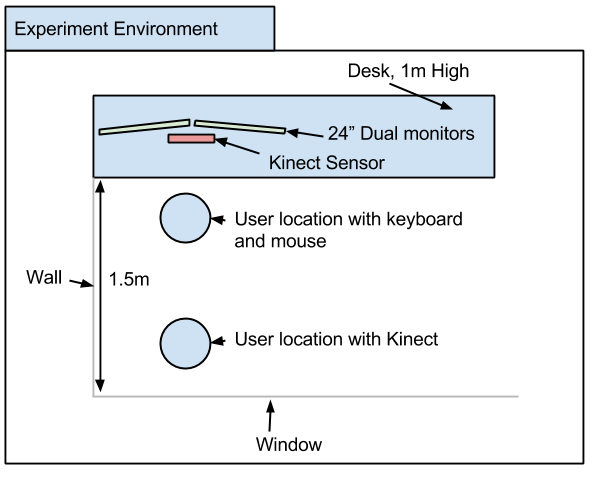
\includegraphics[width=0.8\textwidth]{images/environment.png}
  \caption{Evaluation environment}  
    \label{fig:environment}
\end{figure}


\subsection{Evaluation Method}
A poorly designed experiment will only yield results of limited value, because
of this it was important to ensure that each stage of the experiment was
focused on evaluating a specific area of the visualisation in relation to the
project requirements. There were 3 key methods of gathering results during this
evaluation; a
worksheet to fill out whilst using the visualisation made up of 2 sets of
questions(one for the keyboard \& mouse system and one for the Kinect
system)(APPENDIX), a questionnaire to
fill in afterwards about the experience (APPENDIX), and the examiners
observations about
how the users interacted with the system.  
\\\\
The following are the steps that were carried out during each user evaluation to
ensure that the variables were the same each time
\begin{itemize}
\item The user enters the room and sits down at the computer.
\item They are handed the consent form and information sheet.
\item After these are completed they are handed the user questionnaire and the
set of questions to answer while using the system. On this questionnaire there
are two sets of questions, the first is for the keyboard and mouse system, and
the second if for the Microsoft Kinect system.
\item They are then given a brief introduction into each of the visualisation
components and what the visualisation as a whole represents
\item Following this they are advised that they have 5 minutes to get
familiarised with the system but they do not need to use all of this time (the
amount of time taken will be recorded for analysis of how user friendly and
intuitive the system is).
\item Following this the user is asked to complete the worksheet by first
using the mouse and keyboard system. When they feel they have answered the first
set of questions they will notify the examiner who will move the user to the
Kinect
system to continue with the second set.
\item Once the user has completed both sets of questions they are asked to fill
in the qualitative user questionnaire about their experiences using the
visualisation. 
\item Following this if the examiner has no follow up questions the user is free
to leave.
\end{itemize}

\subsection{Pilot Study}
Due to the significant costs associated with running an experiment, it 
is valuable to conduct a pilot study with one or two 
participants. This allows testing and refining the experimental
design before starting a full-fledged study with numerous 
participants \cite{kosara2003thoughts}. 

The reason for conducting a pilot study for this project was to ensure that
the experiment was
producing the data needed to evaluate the visualisation produced as well
as taking the correct amount of time to complete. In addition to this it was
used to discover whether there were any aspects of the study that would
interfere with the results. One participant was asked to take part in a pilot
study before any results were
collected, this participant is referred to as P1. This participant was asked to
complete all of the activities that
make up the main experiment. This pilot study took approximately 15 minutes as
intended, this included the time needed for the explanation and completion of
paperwork, as well as the experiment itself.

P1 successfully each of the questions whilst using the visualisation with only
limited assistance from the examiner. This assistance was required due to the
wording of
some of the tasks users were asked to complete being ambiguous which caused
unnecessary confusion which could have interfered with the results. These
ambiguous questions and
tasks were removed prior to the main user study. During the main study only P4
and P10 asked for clarification on the questions or tasks.

P1 had some initial difficulty using the range sliders but after a small period
of experimentation began using them for the majority of tasks which turned out
to be very efficient. P1 also found that whist the range sliders were effective,
they did not allow fine enough control for making small changes. The component
of the visualisation that P1 had the most difficulty was using the
view depicting the location of planets in relation to their stars habitable
zones. This difficulty seemed to stem from the lack of a common point of
reference for each planet due to each planet having a different star with its
own habitable zone.

During the Kinect portion of the experiment P1 found that being in a sitting
position whist interacting with the visualisation did not feel natural due to
``being required to reach out and exert effort to hold an upright position of
the arms for an extended period of time''. The following figure displays P1s
reactions to questions about the experience of using the IKVT.
\begin{figure}[H]
  \centering
      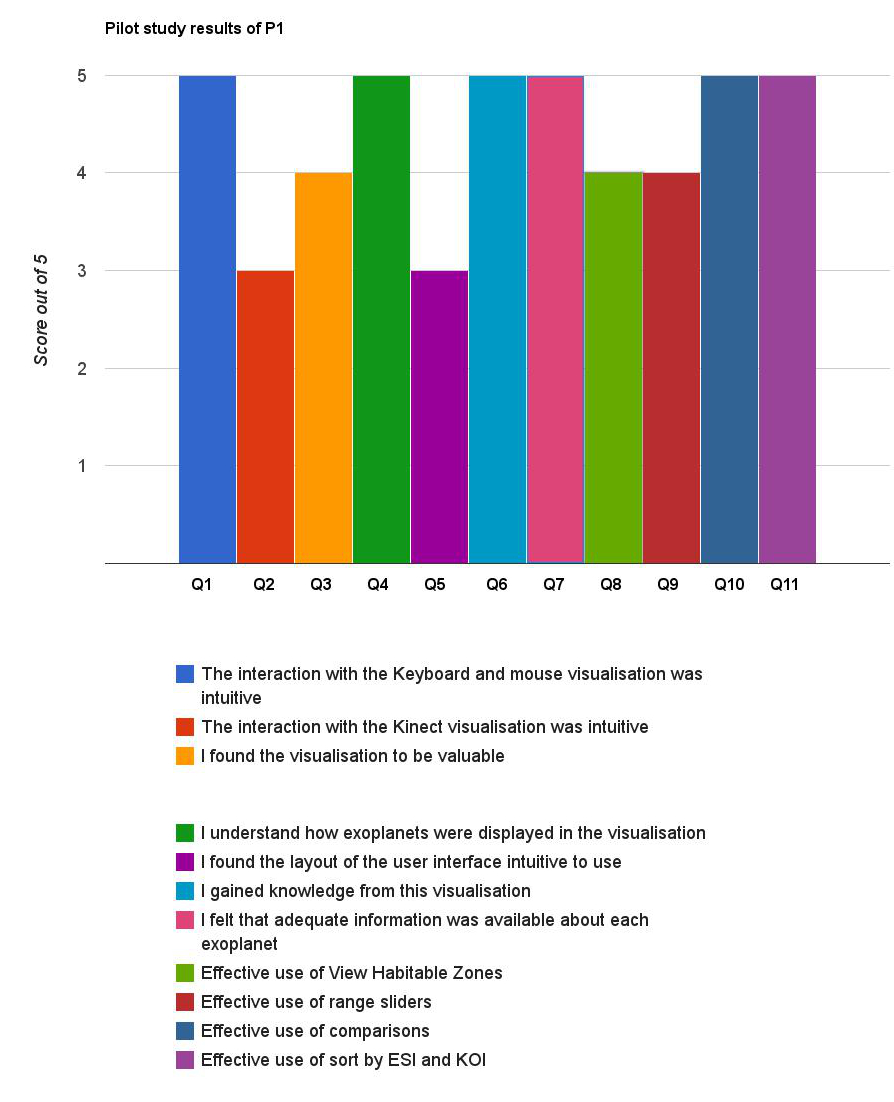
\includegraphics[width=1\textwidth]{images/pilot.jpg}
  \caption{Pilot study results of P1}  
    \label{fig:pilot}
\end{figure}

\section{Results}
The keyboard \& mouse portion of the experiment was primarily intended to
evaluate how the interaction techniques that were introduced into the
visualisation aided users in their information seeking behavior.
This was evaluated through the first part of the worksheet that users filled
in whilst using the visualisation. These questions were designed in a way that
encouraged users to make use of each of the interactive features that was
implemented as part of this project.

The Microsoft Kinect portion of the experiment was intended to evaluate how
users would react to interacting with the visualisation by gesture. The
worksheet for this portion of the evaluation were designed to find out whether
users could successfully navigate the system by gesture.

\subsection{Qualitative Results}
\subsubsection{Evaluation of Functional Requirements}
\begin{enumerate}
{\bf
 \item[R1.] The visualisation needs to display planetary information to convey
knowledge to users.}

The experiment demonstrated that by increasing the amount of information that
was available about each exoplanet, participants were able to effectively access
more
information contained in the Kepler Exoplanet database than in the existing
system. All participants were able to successfully complete the worksheet
questions
that involved accessing information about the exoplanets that was stored in the
text areas contained in the interaction panel.
P8 found that a weakness of the system was the amount of concepts that needed
to be understood about exoplanets planets and so inluding a glossary would be an
improvement. A glossary would allow users to discover the meaning to any of the
wording in the visualisation which would mitigate the risk of users becoming
confused.

All participants reported learning something from the visualisation that they
did not previously know, and those who had no knowledge of exoplanets prior to
the experiment felt that they had learned something valuable. For example P4
felt that using IKVT broadened her perception of how much information we know
about planets so far away.


{\bf
 \item[R2.] The visualisation needs to allow exoplanets to be compared against
one another.}

Whilst all participants used the comparison functionality during the
familiarisation stage, only 3 of the participants used it while completing the
worksheet. This could be because it was not made obvious enough, or because the
questions asked of users did not force them to use this feature to get an
answer. When the participants did use the comparison tool they were able to use
it successfully and most tried it multiple times with multiple exoplanets. P3
found that being able to compare the exoplanets against one another was usefull
as he could leave an interesting exoplanet seleced whilst comparing it against
multiple other exoplanets. He found that it was easy to compare the information
for each exoplanet and to get a sense of the attributes of exoplanets.

{\bf
 \item[R3.] The planets need to be able to be ordered by their similarity to
earth (ESI) and by their Kepler Object of Interest number (KOI).}
 
All participants used the sort by KOI and ESI functionality effectively without
any confusion. P8 liked being able to toggle between the different planetary
sorting and
filter as he found that it gave a clearer view of the attributes in a visual
manner rather than needing to look at the text areas.
P7 found the exoplanets sorted by ESI to be the most interesting view. She
spent
an extended period of time experimenting with this during question 8 of the
worksheet before moving on the later questions. P7 stated that she could find
the potentially habitible planets easily as she could assume that they would
need to be similar to Earth which the visualisation clearly showed.
Successful
 
{\bf \item[R4.] The visualisation needs to allow users to define ranges of
planetary attributes to filter which planets are displayed.}

All participants successfully used the range sliders whilst completing the
worksheet
during the evaluation. The range sliders were heavily used to discover the
exoplanets that were the outliers in regard to their attributes (ie, high
temperatures). 3 out of 10 participants had trouble when moving between
questions on the worksheet due to forgetting
to reset the range sliders after using them and thus only a subset of the
exoplanets were displayed. 
P5 found the zooming effect that occurred when planets were filtered with the
range sliders useful for making more accurate selections and spent time
experimenting with it. P6 found that being able to sort the planets according to
attributes and
then filtering them to remove the planets she did not want was a powerful tool.

{\bf \item[R5.] Users need to be able to view the habitable zones of stars in
relation to the planets orbiting them.}

The evaluation of this requirement showed that whilst the functionality was
successfully implemented it lacked usability. All but one user in the study
found that this was because it was unintuitive. What caused this was that the
habitable zones of each star is different. This meant that each time a user
selected a new exoplanet the location of each of the zones changed as was
intended. However, this confused all but one user as they were expecting the
zones to stay the in the same locations.  

\end{enumerate}

\subsubsection{Evaluation of Nonfunctional Requirements}
\begin{enumerate}
 {\bf\item[R6.] All interaction methods must be visible and intuitive.}
 
The experiment found that all interactive methods were able to be seen and used
by users. However due to the design of the components being low key as to not
draw attention away from the main visalisation, the participants often forgot
about them especially as the interaction panel was at the side of the screen,
for example P5 found that because the information panel was not central in the
visualisation
it required effort to break away from the main visualisation window which broke
the immersion. Another issue found was that the text of the componets in the
interaction was to small for some users to see clearly and quickly.
A common consensus was that the layout of the interactive components were fine
but could be improved by making them “pop out more” especially as many
participants initially spot the text areas changing as planets were selected
until reading the worksheet questions.
 
{\bf \item[R7.] The visualisation must remain uncluttered to reduce information
overload.}

The experiment confirmed that the amount of information displayed in the
visualisation was appropriate for the users tested apart from P7 who felt this
it displayed to much information at once which caused confusion. P10 felt that
the interaction panel contained the right amount of information, but felt that
it could be improved by changing its design to make it stand out more and
emphasise each component contained in it. P4 felt that the names of some of the
attributes were not made clear enough(Eg, ESI, KOI). P5 felt that limiting the
amount that the user could move around in the visualisation by stopping the
camera being able to show to unnecessary places would be an improvement,
especially in the graph view.

{\bf \item[R8.]  There needs to be two modes of interaction with the system,
keyboard and mouse vs gesture based.}

The experiment found that each of the interactive methods had different
strengths and weaknesses. The keyboard \& mouse system was the most effective
for seeking information as it provided more accuracy and was easier to use the
interaction panel. The Microsoft Kinect system was worse for discovering
information, but it was the most fun out of the two options due to its novelty.
All of the users felt that had they had more time with the Kinect system, they
would have been more effective at accessing the information available. This was
because they were preoccupied performing basic actions like moving the camera
and selecting planets due to the short time available. For example P6 found that
she used more time playing around with the Kinect system trying to select
planets rather than trying to get information. All participants but P4 felt that
the visualisation responded the the appropriate actions and magnitudes for each
gesture. P4 felt expected the magnitiute of the visualisation changes to be more
than they were, ie it should have rotated faster. P6 felt that there needed to
be more movement space in which to use the Kinect as some movements felt
cramped. Another weakness discovered about the Kinect sensor was that it
detected the whole hand rather than a more controllable interface like a finger.
Its also found that overlapping planets made it hard to make selections with the
Kinect and that it needed a way to cancel a selection without having to select
another planet.

\end{enumerate}

\subsection{Quantitative Results}
\subsubsection{Evaluation of Functional Requirements}

A key part of this visualisation is that it should be intuitive enough that a
user can walk up to it and feel comfortable using it to explore data within a
short period of time. The results showed that some users felt that they could
effectively use the visualisation very quickly (within 1 to 4 minutes) whilst
others took longer (up to 5 minutes) as Figure \ref{fig:comfort}. 
\begin{figure}[H]
  \centering
      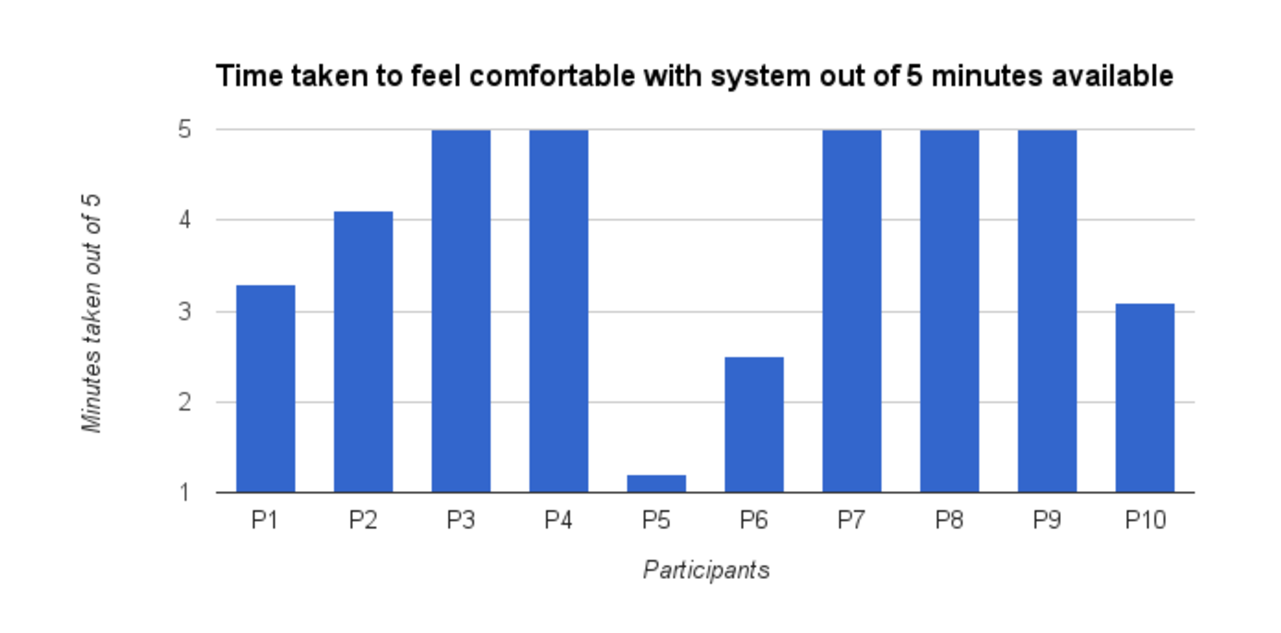
\includegraphics[width=1\textwidth]{images/comfort.pdf}
  \caption{Amount of time taken out of a possible 5 minutes for users to feel
comfortable with
visualisation before moving onto the worksheet. }  
\label{fig:comfort}
\end{figure}

As we can see below in Figure \ref{fig:summary} all users performed well in all
aspects apart from with ``Req: 6 Effectively used habitable zones'' which the
qualitative analysis also found. Another notable result was that the keyboard \&
mouse was rated as more intuitive than the Kinect sensor, again this is
supported by the qualitative results. Apart from these key areas of interest the
results are as expected with each area being scored highly. 
\begin{figure}[H]
\centering
      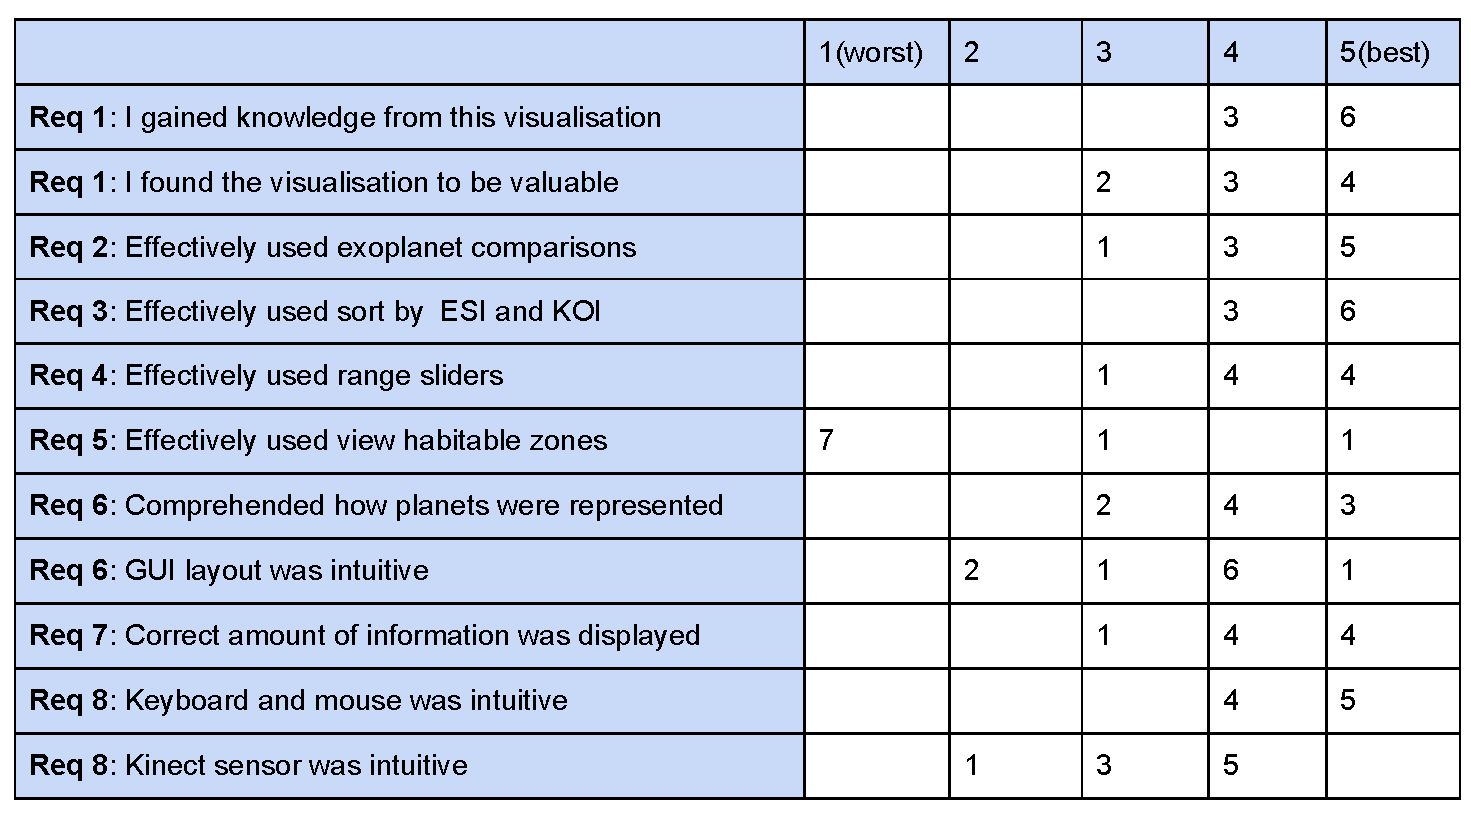
\includegraphics[width=1\textwidth]{images/summaryResults.pdf}
  \caption{Summary of the quantitative results gathered from participants.}  
    \label{fig:summary}
    \end{figure}
    
Seeing how different participants scores attribute to the table in Figure
\ref{fig:summary} helps to understand the distribution of scores. As Figure
\ref{fig:breakdown} shows, some users consistantly gave higher or lower scores
which could have caused a bias in the results. However it does show that some
users enjoyed using the visualisation whilst others did not and the scores
reflect this. 
    
\begin{figure}[H]
  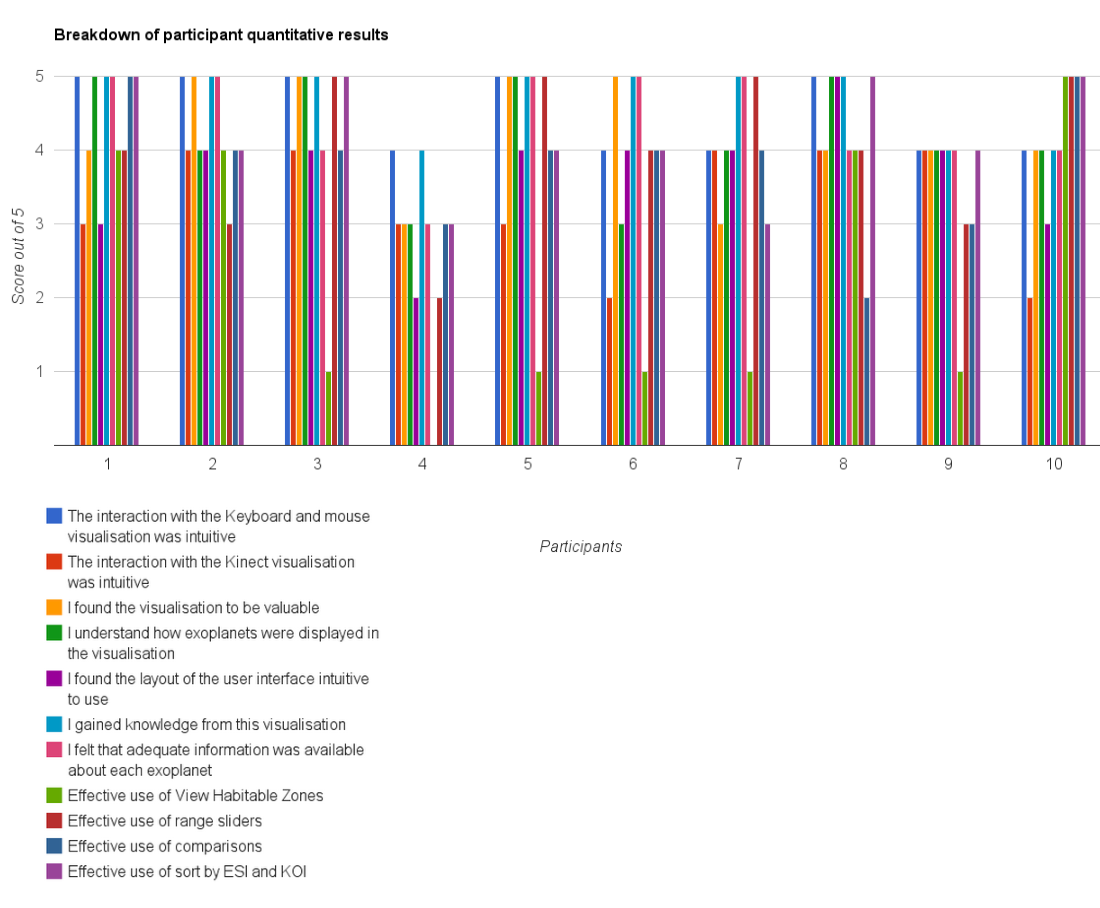
\includegraphics[width=1\textwidth]{images/breakdown.pdf}
  \caption{Breakdown of quantitative results between users}  
    \label{fig:breakdown}
\end{figure}

\section{Discussion}
\subsection{Threats to Validity}
A key factor in this user evaluation is the small number of users which was
chosen due to the time limit of 300 hours which did not allow for a larger more
in depth study. Because of this, the results gathered from this evaluation may
not be representative of a larger population. It was also limited to a narrow
demographic of you professionals and students which does not cover all of the
intended users of IKVT. To amend this the population of this study would need to
be expanded to contain age ranges above and below those in this study.

A further threat to the validity of this evaluation was the limit placed on
participants for the familiarisation stage. Some participants may have required
even more time than the 5 minutes alloted for. By cutting the familiarisation
stage off at this point it may have caused some participants to be unprepared
for carry out the completion of the worksheet and thus skewing the results.

\subsection{Potential Improvments}
Due to the negative results surrounding the viewing of the habitable zones of
stars,
this area of the evaluation should be analysed further to determine whether the
tasks in the evaluation relating to it were flawed, or whether the functionality
and its design were flawed. To discover this it would be important to revaluate
the questions asked of user revolving around this functionality. Following this
it would be possible to determine if the the functionality needed to be
redesigned. 


\section{Summary of Evaluation}
This evaluation of IKVT provided several key results and insights into the
success of this project. The general consensus by the participants of the study
was that the system had a low learning curve, was enjoyable to use, and allowed
access to interesting information. There was also a common consensus among the
participants that the Kinect system was more fun to use than the keyboard \&
mouse because of its novelty, but lacked the control that the
keyboard \& mouse allowed which made it less effective at accessing the
information in the visualisation. The keyboard \& mouse was found to the be the
most effective method for nagivating the visualisation because of the amount of
control that it offered users as well as being the interactive medium that
participants had the most experience with.

The evaluation revealed one problem area in the visualisation that was related
to Requirement 5 (Users need to be able to view the habitable zones of stars in
relation to the planets orbiting them), and Requirement 6 (All interaction
methods must be visible and intuitive). This problem was that users found that
viewing where each exoplanet was located in relation to their stars habitable
zones was unintuitive and difficult to use. This result could have occured for a
range of reasons, the most likely being that the evaluation questions were
counterproductive to using this funtionality, or that the functionality itself
is flawed.

This user study served to evaluate how effectively IKVT could convey the
information in the Kepler Exoplanet dataset. The findings all pointed to it
being successfull in this regard. However, there are areas that this evaluation
could be improved to strengthen this result. The main improvement for this
evaluation is to include a larger number of participants more representative of
the wider population.



